%%=============================================================================
%% Comparison between Linux and Windows agents
%%=============================================================================

\chapter{Comparison}%
\label{ch:comparison}

\section{Introduction}%
\label{sec:introduction-comparison}
In this chapter, we will compare the Linux and Windows agents. The comparison will be executed on a TeamCity instance with a Linux agent and Windows agent. The comparison will give some insights into the performance of the agents and their energy-efficiency.

\section{TeamCity cloud}%
\label{sec:teamcity-cloud}
To start my comparative analysis I had some requirements such as a TeamCity instance, a Linux agent and a Windows agent. After some research I found out that Jetbrains offers a cloud version of TeamCity \autocite{Bevan2021}. This cloud version is free for 3 agents and 100 build configurations. This was perfect for my research since I only needed 2 agents. 

\section{Agents}
For my agents I used two virtual machines from Azure to ensure that the agents were provided by the same cloud provider and also to avoid other factors that could influence the results. For the Windows agent I used Windows 10 and for the Linux agent I used Ubuntu 20.04. The agents were configured with the same specifications to ensure a fair comparison. TeamCity Cloud came with some pre-installed agents but this came with a limited amount of builds and virtual machines made it possible to have more control over the agents.

\section{Builds}
To compare the agents I created a build configuration for each operating system so it was easy to seperate the right builds. The builds were the same for both agents. The first build configuration ran on the agents was a matrix operation. This would need some CPU power and memory to run. The second build configuration was a matrix multiplication. In following image you can see the dashboard of the TeamCity instance with the two build configurations.

\begin{figure}[H]
\centering
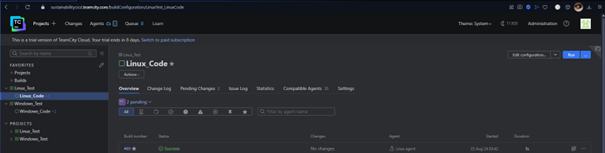
\includegraphics[width=0.8\textwidth]{graphics/TeamCity.png}
\caption{TeamCity dashboard with the two build configurations}
\end{figure}

\section{Metrics}
The two most important factors in terms of energy-efficiency are the CPU usage and the memory usage. The used memory is measured by implementing it in the build configuration. The CPU usage was a lot more difficult to measure. Through a script that I manually started before running the build it measured the CPU usage for the following 60 seconds. This way, it was possible to measure the average CPU usage an interval where the build was running. By doing this for every build, it was possible to compare the CPU usage of the Linux and Windows agent.

\section{Results}
The results of the comparison can be found in the following sections. The results are based on the the CPU usage and the memory usage of the agents.

\subsection{Experiment 1: Matrix operation}
In the following tables you can find the results of the matrix operation on the Linux and Windows agent. We can immediately see that the CPU usage is higher on the Linux agent compared to the Windows agent. The memory usage is also a little bit higher on the Linux agent. The builds on the Windows agent are more consistent compared to the Linux agent.
\begin{table}[H]
\centering
\begin{tabular}{|l|l|l|l|}
\hline
Build nr & Build time & CPU usage & Memory usage \\ \hline
1        & 12s        & 46,39\%   & 72,00       \\ \hline
2        & 12s        & 41,51\%   & 72,19       \\ \hline
3        & 12s        & 45,06\%   & 72,00       \\ \hline
4        & 12s        & 35,74\%   & 72,13       \\ \hline
5        & 12s        & 35,91\%   & 72,00       \\ \hline
\end{tabular}
\caption{Results of the matrix operation on the Linux agent}
\end{table}

\begin{table}[H]
\centering
\begin{tabular}{|l|l|l|l|}
\hline
Build nr & Build time & CPU usage & Memory usage \\ \hline
1        & 12s        & 29,56\%   & 67,11       \\ \hline
2        & 12s        & 29,37\%   & 67,39       \\ \hline
3        & 12s        & 29,40\%   & 67,31       \\ \hline
4        & 12s        & 29,20\%   & 67,37       \\ \hline
5        & 12s        & 29,42\%   & 67,38       \\ \hline
\end{tabular}
\caption{Results of the matrix operation on the Windows agent}
\end{table}

\subsection{Experiment 2: Matrix multiplication}
In the following tables you can find the results of the matrix multiplication on the Linux and Windows agent. This second experiment shows the same results as the first experiment. The CPU usage is higher on the Linux agent compared to the Windows agent. The memory usage is also a little bit higher on the Linux agent. The consistency of the builds on the Windows agent is better compared to the Linux agent. This shows that a Windows agent is more energy-efficient compared to a Linux agent.
\begin{table}[H]
\centering
\begin{tabular}{|l|l|l|l|}
\hline
Build nr & Build time & CPU usage & Memory usage \\ \hline
1        & 5s         & 35,00\%   & 15,14       \\ \hline
2        & 5s         & 35,98\%   & 15,26       \\ \hline
3        & 5s         & 31,38\%   & 15,08       \\ \hline
4        & 5s         & 27,85\%   & 15,2        \\ \hline
5        & 5s         & 32,03\%   & 15,08       \\ \hline
\end{tabular}
\caption{Results of the matrix multiplication on the Linux agent}
\end{table}

\begin{table}[H]
\centering
\begin{tabular}{|l|l|l|l|}
\hline
Build nr & Build time & CPU usage & Memory usage \\ \hline
1        & 5s         & 29,54\%   & 7,63        \\ \hline
2        & 5s         & 29,65\%   & 7,66        \\ \hline
3        & 5s         & 29,65\%   & 7,66        \\ \hline
4        & 5s         & 30,04\%   & 7,62        \\ \hline
5        & 4s         & 29,59\%   & 7,61        \\ \hline
\end{tabular}
\caption{Results of the matrix multiplication on the Windows agent}
\end{table}
